% Clever thing to minimize the files I need to edit to change how the files are
% looking. The following one line comment is to trick VIM-LaTeX
\documentclass{scrartcl}
%documentclass{scrartcl}
\KOMAoptions{
    fontsize=10pt
}
\setkomafont{pagenumber}{\bfseries\upshape\oldstylenums}
\renewcommand{\titlefont}{\rm\bfseries\LARGE}
\usepackage{
    ifxetex, 
    ifdraft,
    ifthen
}

\ifxetex
  \usepackage{fontspec}
  \usepackage{xunicode}
  \defaultfontfeatures{Mapping=tex-text} % To support LaTeX quoting style
  \setromanfont{Gentium}
\else
  \usepackage[utf8]{inputenc}
  \usepackage[T1]{fontenc}
  \usepackage{lmodern,textcomp}
\fi

\usepackage{
%    standalone,
%    lastpage,
    geometry,
    scrpage2,
%    setspace,
    amsmath,
    caption,
    calc,
%    floatrow,
}
\usepackage{
%    xcolor,
    graphicx,
    tikz,
    chemfig
}
\usepackage[final]{listings}
\usepackage[version=3]{mhchem}
\usepackage[update,verbose=false]{epstopdf}
\usepackage[colorinlistoftodos,obeyDraft]{todonotes}
\usepackage{hyperref}


% Set the geometry
\geometry{
    paper = a4paper,
    top=3cm,
    bottom=4cm,
    footskip=1cm,
    marginparwidth=3.5cm,
    headsep=1cm
}
\ifoptiondraft{
\geometry{inner=1.5cm, outer=4cm}
}{
\geometry{inner=3.0cm, outer=2.5cm}
}

%\onehalfspacing

% Setup hyperref
\hypersetup{
    colorlinks,
    urlcolor=blue,
    breaklinks
}

\usetikzlibrary{
    arrows,
    decorations.pathmorphing,
    backgrounds,
    positioning,
    fit,
    petri
}

% Define collors
\definecolor{myyellow}{HTML}{FFFAC9}
\definecolor{myyellowl}{HTML}{FFFBDD}

% Define lstlisting env
\lstset{
    language=[LaTeX]TeX,
    backgroundcolor=\color{myyellowl},
    numbers=left,
    numberstyle=\footnotesize,
    breaklines=true,
    breakatwhitespace=true,
    print=true
}

% Renew 2 styles
\renewpagestyle{plain}{{}{}{}}{{}{}
{\hfill\pagemark{}}}
\renewpagestyle{headings}{{}{}{}}{{}{}
{\hfill\pagemark{}}}

% Set the headings page style
\pagestyle{headings}

% Text mode commands
\newcommand{\uurl}[2]{\href{#1}{#2}\footnote{The URL is \url{#1}}}
\newcommand{\ftype}[1]{\texttt{.#1}}
\newcommand{\fname}[2]{\texttt{#1.#2}}
\newcommand{\pkg}[1]{\texttt{#1}}
\newcommand{\env}[1]{\texttt{#1}}
\newcommand{\cmd}[1]{\texttt{\textbackslash{}#1}}
\newcommand{\usepkg}[2]{
    \texttt{\textbackslash{}usepackage%
    \ifthenelse{\equal{#2}{}}{}{[#2]}\{#1\}}}
\newcommand{\comment}[1]{}

% New commands which ease the work. Units and relative uncertainties
\newcommand{\unit}[1]{\ensuremath{\, \mathrm{#1}}}
\newcommand{\rel}[1]{\ensuremath{ \cfrac{\Delta #1}{#1}}}
\newcommand{\eten}[1]{\ensuremath{ \times 10^{#1}}}
\newcommand{\DP}[2]{\ensuremath{\cfrac{\partial #1}{\partial #2}}}
\newcommand{\DD}[2]{\ensuremath{\cfrac{\mathrm{d} #1}{\mathrm{d} #2}}}
\newcommand{\dd}[1]{\ensuremath{\mathrm{d}#1}}

% Alter some LaTeX defaults for better treatment of figures:
    % See p.105 of "TeX Unbound" for suggested values.
    % See pp. 199-200 of Lamport's "LaTeX" book for details.
    %   General parameters, for ALL pages:
    \renewcommand{\topfraction}{0.9}    % max fraction of floats at top
    \renewcommand{\bottomfraction}{0.8} % max fraction of floats at bottom
    %   Parameters for TEXT pages (not float pages):
    \setcounter{topnumber}{2}
    \setcounter{bottomnumber}{2}
    \setcounter{totalnumber}{4}     % 2 may work better
    \setcounter{dbltopnumber}{2}    % for 2-column pages
    \renewcommand{\dbltopfraction}{0.9} % fit big float above 2-col. text
    \renewcommand{\textfraction}{0.07}  % allow minimal text w. figs
    %   Parameters for FLOAT pages (not text pages):
    \renewcommand{\floatpagefraction}{0.7}      % require fuller float pages
    % N.B.: floatpagefraction MUST be less than topfraction !!
    \renewcommand{\dblfloatpagefraction}{0.7}   % require fuller float pages

\captionsetup{
    format          = plain,        %
    labelformat     = simple,       %
    labelsep        = period,       %
    justification   = default,      %
    font            = default,      %
    labelfont       = {bf,sf},      %
    textfont        = default,      %
    margin          = 0pt,          %
    indention       = 0pt,          %
    parindent       = 0pt,          %
    hangindent      = 0pt,          %
    singlelinecheck = false         %
}

\renewcommand{\thefigure}{\oldstylenums{\arabic{figure}}}

\setatomsep{5mm}
\setbondoffset{.5mm}
\setcrambond{2.5pt}{1pt}{2pt}
\setbondstyle{thick}
\renewcommand*\printatom[1]{{\footnotesize\ensuremath{\mathsf{#1}}}}


% Custom packages
\newcommand{\hho}{\ensuremath{\mathrm{H_2O}}}
\newcommand{\un}[1]{\unit{#1}}

\newcounter{chemcmp}
\newcounter{chemcmpp}
\renewcommand{\thechemcmp}{\arabic{chemcmp}}
\renewcommand{\thechemcmpp}{\alph{chemcmpp}}
\newcommand{\cmpinc}{
    \refstepcounter{chemcmp}
    \setcounter{chemcmpp}{0}
}
\newcommand{\cmp}[1]{
    \cmpinc
    \textbf{\thechemcmp }
    \label{#1}
}
\newcommand{\cmppe}[1]{
    \refstepcounter{chemcmpp}
    \textbf{\thechemcmp\thechemcmpp }
    \label{#1}
}
\newcommand{\cmppn}[1]{
    \cmpinc
    \refstepcounter{chemcmpp}
    \textbf{\thechemcmp\thechemcmpp }
    \label{#1}
}

\usepackage{graphicx}
\graphicspath{{./figs/}}
\usepackage[update,verbose=false]{epstopdf}
\usepackage{tikz}
\newlength{\tikzunit}

\title{Defining your own macros, commands and environments}
\author{Ignas Anikevicius}

\begin{document}

\maketitle

\begin{abstract}
    This is one of the most useful \TeX\ features. Actually all \LaTeX\ system
    is just a set of macros and environments to extend \TeX\ features.
    Definition of your own commands might look a very difficult thing to do, but
    actually it is not! I will examine some examples in the following sections
\end{abstract}

\tableofcontents

\section{Defining new \LaTeX\ commands}

For example, we want to have a command named \verb|titleoftheproject| and we
want it to return the title of our current project, w

Let's now consider a situation where a person is writing a dissertation on the
physical properties of water and he uses its chemical formula $\left( \hho
\right)$ a lot. It takes time to typeset such a formula, and the code actually
looks like this: \verb|$\mathrm{H_2O}$|. However, if we have
something similar to the following code in the preamble, we could just write
\verb|\hho|.
\begin{lstlisting}
\newcommand{\hho}{\ensuremath{\mathrm{H_2O}}}
\end{lstlisting}

The best place to get all the necessary knowledge for being able to do the same
as was done above would be 
\href{https://secure.wikimedia.org/wikibooks/en/wiki/LaTeX/Customizing_LaTeX#New_commands}{this
page}. There you will be able to find simpler examples and much more examples.

Here I will just give you some useful code snippets, which might give you some
ideas or turn out to be useful.

\subsection{Typesetting units correctly}

Well typeset document will usually have very elegant code. Which means, that for
example to enter an equation one will not switch back and forth from the
\verb|math| mode, but rather enter everything there. However, if units are
typeset right away, they might appear in italics (ie. the same way as the
equation variables appear), which is not what we want.

There are several packages which might be worth looking, but I find it just
unnecessary as one can solve this issue with only one short command.

Let's consider a following expression:
\[
    m = \rho \times V 
      = 1000 \, \mathrm{kg \cdot m^{-3}} 
      \times 3 \, \mathrm{m^{-3}} 
      = 3000 \, \mathrm{kg}
\]

and the code for it can be found bellow:
\lstinputlisting{units-without.tex}

Now look at the equation generated by another version of the code where we do
not enter all those tedious commands:
\[
    m = \rho \times V 
      = 1000 \un{kg \cdot m^{-3}} 
      \times 3 \un{m^{-3}} 
      = 3000 \un{kg}
\]

\lstinputlisting{units.tex}

This can be achieved with the following command in the preamble of the file.
\begin{lstlisting}
\newcommand{\un}[1]{\ensuremath{\, \mathrm{#1}}}
\end{lstlisting}

You might wonder, why to use a newly defined command, if the amount of code
does not decrease very much. However, you \textbf{should} think about the case
where you would like to change the formatting of the units just ever so slightly
and if you used the \verb|\un| command, which you had defined previously, you
would need to change only one line, but otherwise you would need to change the
entire document, which I believe is not the fastest way to do it.

\subsection{Typesetting lengthy and tedious expressions quickly}

This probably might apply more to people who are dealing with uncertainties more
and need to write expressions which are quite repetitive in a sense. Here is an
example with relative fractions.

Suppose we have the following the equations:
\begin{align*}
    p &= \cfrac{mRT}{MV}
    \\
    \rel{p} &= \rel{m} + \rel{T} + \rel{V}
\end{align*}


Please notice, that the relative errors do have very repetitive expressions,
as we always have a fraction and the symbol is repeated twice in the numerator
and denumerator, just on the numerator there is an extra $\Delta$ symbol in
front.

Now let's compare two possible ways to achieve the above line for the fractional
errors:
\lstinputlisting{relfrac-without.tex}
\lstinputlisting{relfrac.tex}

I guess you can see how much more readable the second variant is. And it is
achieved by defining the \verb|\rel| command in the preamble:
\begin{lstlisting}
\newcommand{\rel}[1]{\ensuremath{\cfrac{\Delta #1}{#1}}}
\end{lstlisting}


\section{Counters and more elaborate commands}

Since we now how to define new commands in \LaTeX{} and ease our life in this
way, we can now go one step further. Suppose we have a large document with a lot
of figures and in those figures we have a lot of structures, which we would like
to number and refer easily in the text. 

\subsection{Example}

So defining compound \cmp{cmp:benzene} and \cmp{cmp:naphtalene} is
very easy.  Referencing them (Compound \ref{cmp:naphtalene} and
\ref{cmp:benzene}) is also easy.
Look at the figure \ref{fig:compeg} to see how you can incorporate it
into figures.

\begin{figure}[h]
    \centering
    \setlength{\tikzunit}{.085\textwidth}
    \begin{tikzpicture}[scale=1.0,x=\tikzunit,y=\tikzunit]
% ---- Draw a grid which should help to position things -----------
%        \draw[step= .5,color=gray,thin,dashed] (-4,-4) grid (4,4);
%        \draw[step=1.0,color=gray]             (-4,-4) grid (4,4);
%        \draw[step=4.0,color=black]            (-4,-4) grid (4,4);
%  Notes:
%       just uncomment the lines with draw commands and the grid
%       will appear.  The commands, I believe are self explanatory
%       and it can be drawn as big as you want. The two coordinates
%       denote lower left and upper right corners of the grid.
% -----------------------------------------------------------------
        \node(0,0){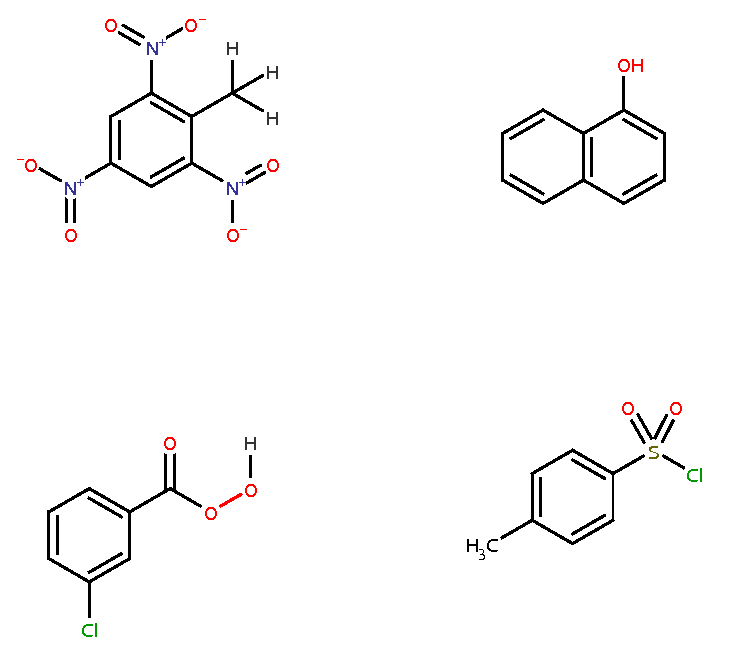
\includegraphics[width=7\tikzunit]{4struct.eps}};
        \draw ( 2.1, 0.5) node{\cmp{cmp:naphtol}};
        \draw (-2.1, 0.5) node{\cmp{cmp:TNT}};
        \draw (-2.1,-3.5) node{\cmp{cmp:mCPBA}};
        \draw ( 2.1,-3.5) node{\cmp{cmp:TsCl}};
    \end{tikzpicture}
    \caption{Overlaying \LaTeX{} commands on top of the figure. To
    get the correct numbers we used a newly created
    \texttt{cmp} command. As you see the order of the numbers is
    determined by the order of code execution.}
    \label{fig:compeg}
\end{figure}

\lstinputlisting{compnum.tex}

The \verb|\cmp| command definition is as follows:
\begin{lstlisting}
\newcounter{chemcmp}
\renewcommand{\thechemcmp}{\arabic{chemcmp} }
\newcommand{\cmp}[1]{\refstepcounter{chemcmp}
    \textbf{\thechemcmp}
    \label{#1}}
\end{lstlisting}

\subsection{Example 2}

Now we can extend the idea of numbering the compounds and including numbers like
1a, 1b. I will use the same for structures, just I will change the numbers.

\begin{figure}[h]
    \centering
    \setlength{\tikzunit}{.085\textwidth}
    \begin{tikzpicture}[scale=1.0,x=\tikzunit,y=\tikzunit]
% ---- Draw a grid which should help to position things -----------
%        \draw[step= .5,color=gray,thin,dashed] (-4,-4) grid (4,4);
%        \draw[step=1.0,color=gray]             (-4,-4) grid (4,4);
%        \draw[step=4.0,color=black]            (-4,-4) grid (4,4);
%  Notes:
%       just uncomment the lines with draw commands and the grid
%       will appear.  The commands, I believe are self explanatory
%       and it can be drawn as big as you want. The two coordinates
%       denote lower left and upper right corners of the grid.
% -----------------------------------------------------------------
        \node(0,0){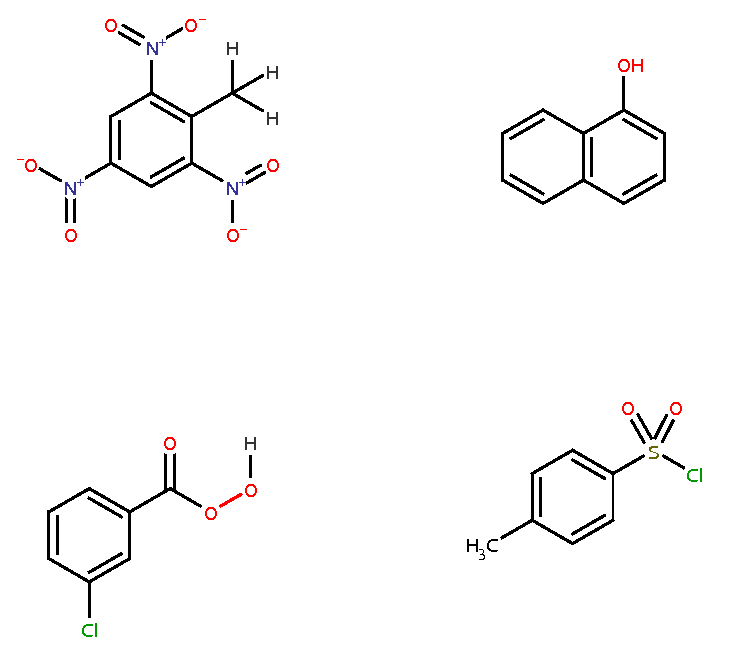
\includegraphics[width=7\tikzunit]{4struct.eps}};
        \draw (-2.1, 0.5) node{\cmp{cmp:TNT1}};
        \draw ( 2.1, 0.5) node{\cmppn{cmp:napht-2-ol1}};
        \draw (-2.1,-3.5) node{\cmppe{cmp:mCPBA1}};
        \draw ( 2.1,-3.5) node{\cmppe{cmp:TsCl1}};
    \end{tikzpicture}
    \caption{Overlaying \LaTeX\ commands to get some nice things.}
    \label{fig:compegg}
\end{figure}

\lstinputlisting{fig.tex}

The \verb|\cmp| name stands for the 'compound'
whereas \verb|\cmppn| is for 'subcompound new' and \verb|\cmppe| is for
'subcompound existing'. The reason why I have made 2 commands for 'subcompounds'
is that one is for the entry of the first 'subcompound' (e.g. 1a) and the other
compound is for adding 'subcompounds' (e.g. 1b, 1c, 1d\ldots).
The code in the preamble defining the commands \verb|\cmp|, \verb|\cmppn|,
\verb|\cmppe| is as follows:
\begin{lstlisting}
\newcounter{chemcmp}
\newcounter{chemcmpp}
\renewcommand{\thechemcmp}{\arabic{chemcmp}}
\renewcommand{\thechemcmpp}{\alph{chemcmpp}}
\newcommand{\cmpinc}{
    \refstepcounter{chemcmp}
    \setcounter{chemcmpp}{0}
}
\newcommand{\cmp}[1]{
    \cmpinc
    \textbf{\thechemcmp }
    \label{#1}
}
\newcommand{\cmppe}[1]{
    \refstepcounter{chemcmpp}
    \textbf{\thechemcmp\thechemcmpp }
    \label{#1}
}
\newcommand{\cmppn}[1]{
    \cmpinc
    \refstepcounter{chemcmpp}
    \textbf{\thechemcmp\thechemcmpp }
    \label{#1}
}
\end{lstlisting}

\end{document}

% Editor configuration:
% vim: tw=80:spell:spelllang=en_gb


